\documentclass{article}
\usepackage{graphicx}
\usepackage{amsmath}
\usepackage{amssymb}
\usepackage[italicdiff]{physics}
\usepackage{enumerate}
\usepackage{microtype}
\DisableLigatures{encoding= *, family=*}
\usepackage{titlesec}
\usepackage{xfrac}
\setcounter{secnumdepth}{4}
\usepackage{xcolor}
\usepackage[bookmarks=false]{hyperref}
\usepackage{mathtools}
\usepackage{tikz} 
\newcommand*\fullcirc[1][0.3ex]{\tikz\fill (0,0) circle (#1);} 
\usepackage{bigints}
\hypersetup{
    colorlinks=true,
    linkcolor=[RGB]{59 108 209},
    urlcolor=[RGB]{59 108 209}
}
\urlstyle{same}

\titleformat{\paragraph}
{\normalfont\normalsize\bfseries}{\theparagraph}{1em}{}
\titlespacing*{\paragraph}
{0pt}{3.25ex plus 1ex minus .2ex}{1.5ex plus .2ex}

\title{Photo Halogenation}
\author{}
\date{}

\begin{document}
\maketitle

\section{Reaction and Mechanism}
\begin{center}
    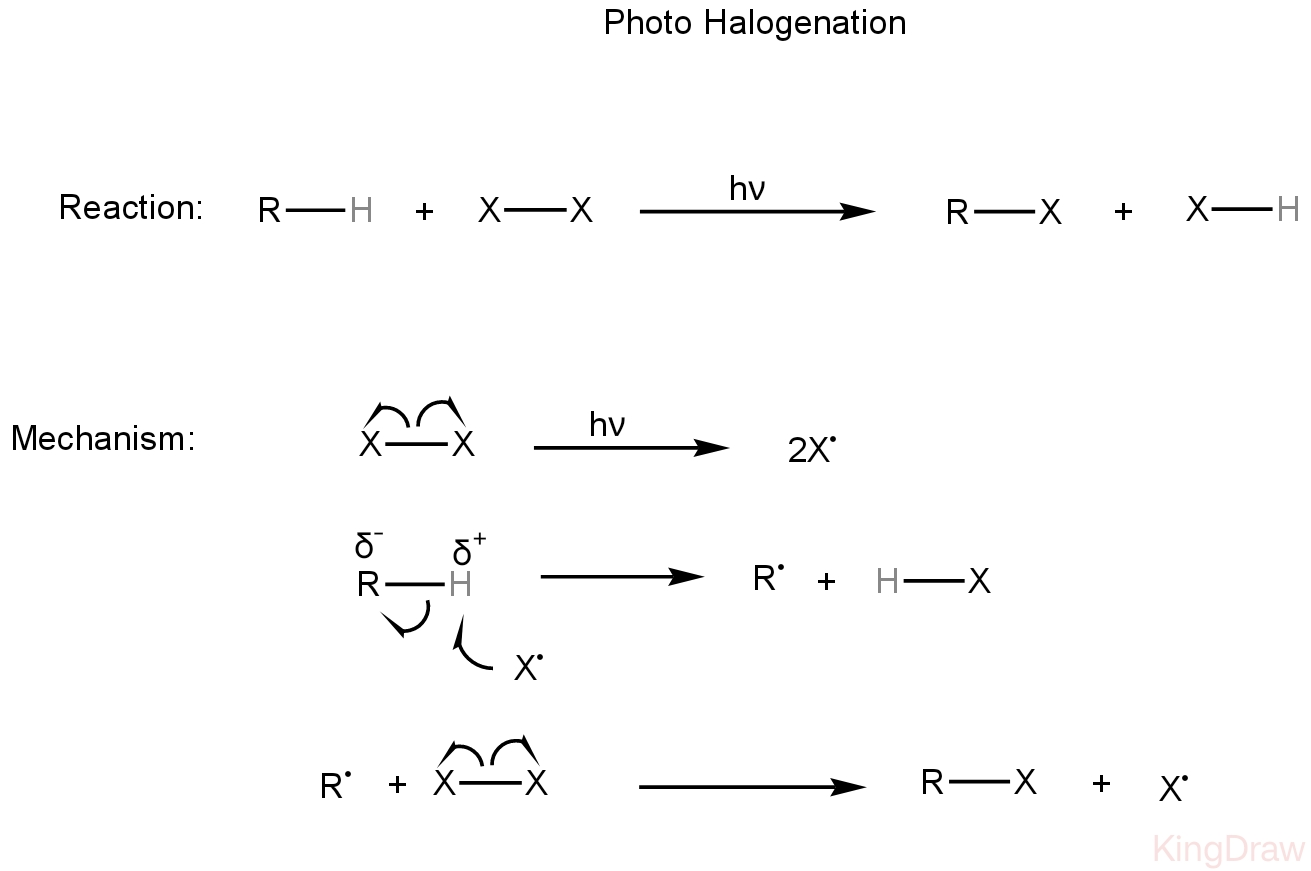
\includegraphics[scale=0.3]{PhotoHalogenanion_1722173018626.JPEG}
\end{center}

\section{Reaction Observations}
\begin{enumerate}[i.]
    \item $C^{\fullcirc}$ obtained as intermediate.
    \item Example of $C^{\fullcirc}$ substitution reaction.
    \item Kinetic isotopic effect is observed.
    \item Example of Oxidation reaction.
    \item Formation of $C^{\fullcirc}$ is RDS.
    \item $ROR \propto \textit{ Stability of } C^{\fullcirc}$
    \item $ROR$ for $X_{2}$, $F_{2}>Cl_{2}>Br_{2}>I_{2}$
\end{enumerate}
\end{document}